\documentclass[11pt]{beamer}
\usetheme{Boadilla}
\usepackage[utf8]{inputenc}
\usepackage[spanish]{babel}
\usepackage{amsmath}
\usepackage{amsfonts}
\usepackage{amssymb}
\usepackage{graphicx}
\usepackage{subfig}
\usepackage{natbib}

%%%%% Color institucional
\definecolor{MyBackground}{rgb}{1.0000,0.9451,0.6549}
\definecolor{itesm}{HTML}{0658a6}
\definecolor{lnppdos}{RGB}{59,124,188}
\definecolor{lnpptres}{RGB}{124,172,212}
%\definecolor{MyBackground}{RGB}{255,241,167}
%\setbeamercolor{background canvas}{bg=MyBackground}
\setbeamercolor*{palette primary}{bg=lnpptres, fg = black}
\setbeamercolor*{palette secondary}{bg=lnppdos, fg = white}
\setbeamercolor*{palette tertiary}{bg=itesm, fg = white}
\setbeamercolor{frametitle}{fg=itesm,bg=white}
\setbeamercolor{title}{fg=white,bg=itesm}
\setbeamercolor{caption name}{fg=itesm}
\setbeamercolor*{item}{fg=itesm}
\usepackage{xcolor}

%%%%%%
\title[]{Virtualización y Contenedores en Cómputo Científico}
\institute[ITESM]{Data Pub\\ ITESM} 
\date{\today} 
\subject{Resultados} 
\titlegraphic{
\includegraphics[width=3cm]{images/itesm}\hspace*{7.5cm}
}
%\title{Turing ODE}
%\setbeamercovered{transparent} 
%\setbeamertemplate{navigation symbols}{} 
%\logo{} 
%\institute{} 
%\date{} 
%\subject{} 
\begin{document}

\begin{frame}
\titlepage
\end{frame}

%\begin{frame}
%\tableofcontents
%\end{frame}

\begin{frame}{Centros de Super Cómputo}
	\begin{figure}
		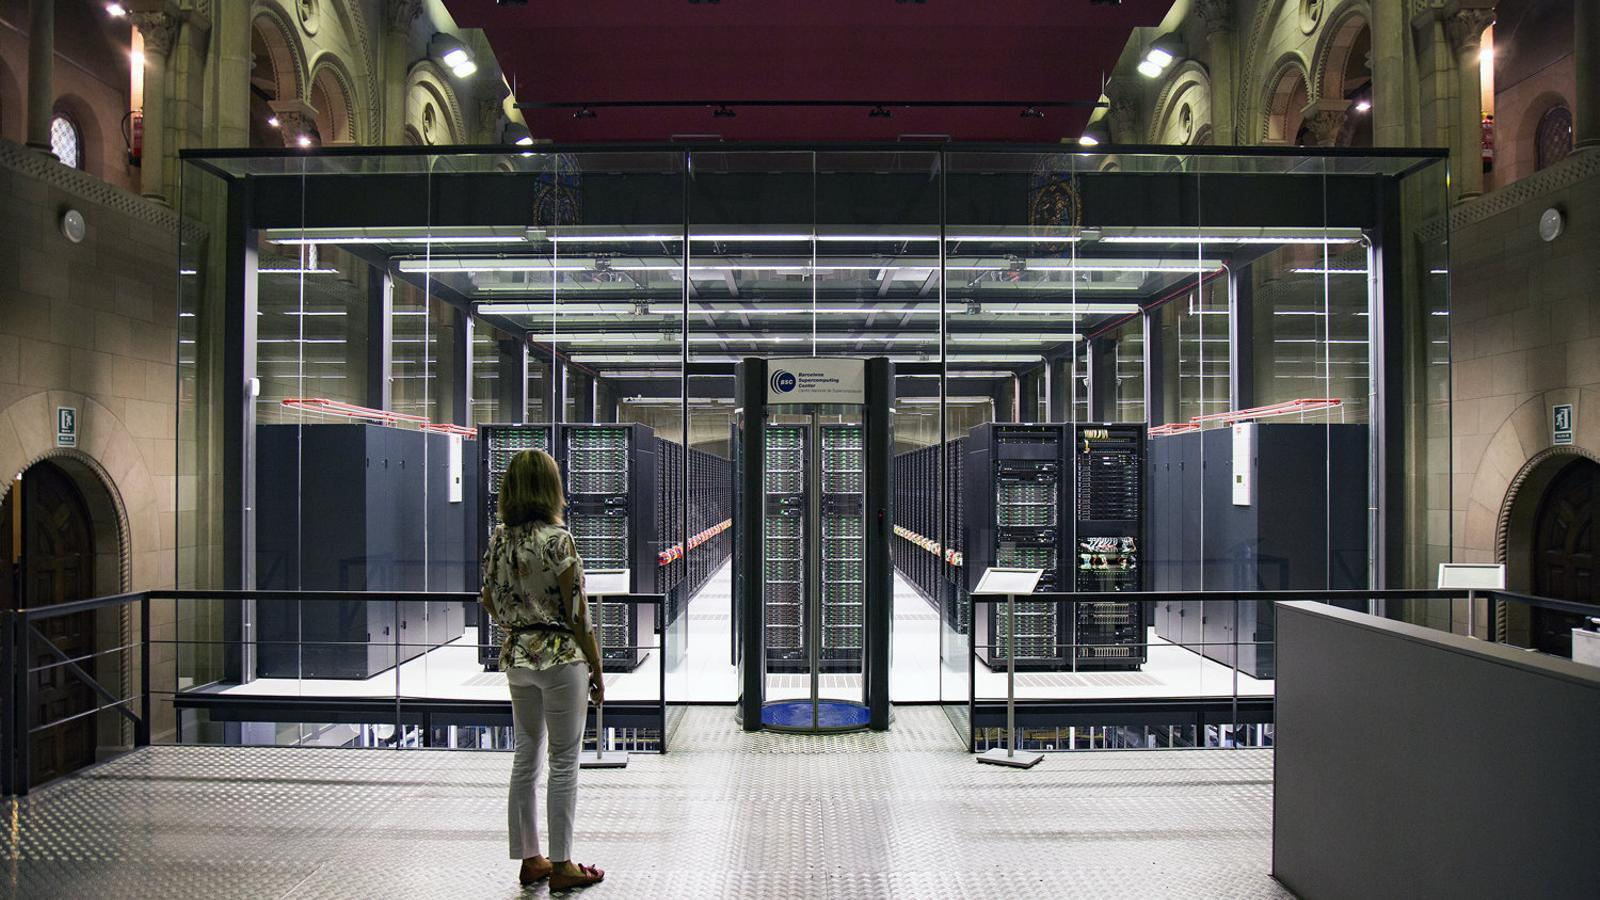
\includegraphics[scale=0.2]{images/barcelona_supercomputing.jpg}
		\caption{Barcelona Supercomputing Center}
	\end{figure}
\end{frame}

\begin{frame}{Centros de Super Cómputo}
	\begin{center}
		\textbf{Centros de Super Cómputo : Recurso compartido}
	\end{center}
	
	\begin{itemize}
		\item  \textbf{Usuaria-Clienta}. Relacionadas con un grupo o institución.
		\item \textbf{Administradoras}. Satisfacen distintas necesidades de las clientas:
			\begin{itemize}
				\item Versiones de software.
				\item Compiladores.
				\item Módulos.
				\item Sistemas de archivos.
				\item Permisos.
			\end{itemize}
		
	\end{itemize}

\end{frame}

\begin{frame}{Arquitectura de un Cluster de HPC (High Perfomance Computing)}
	\vspace{-0.9cm}
	\begin{figure}
		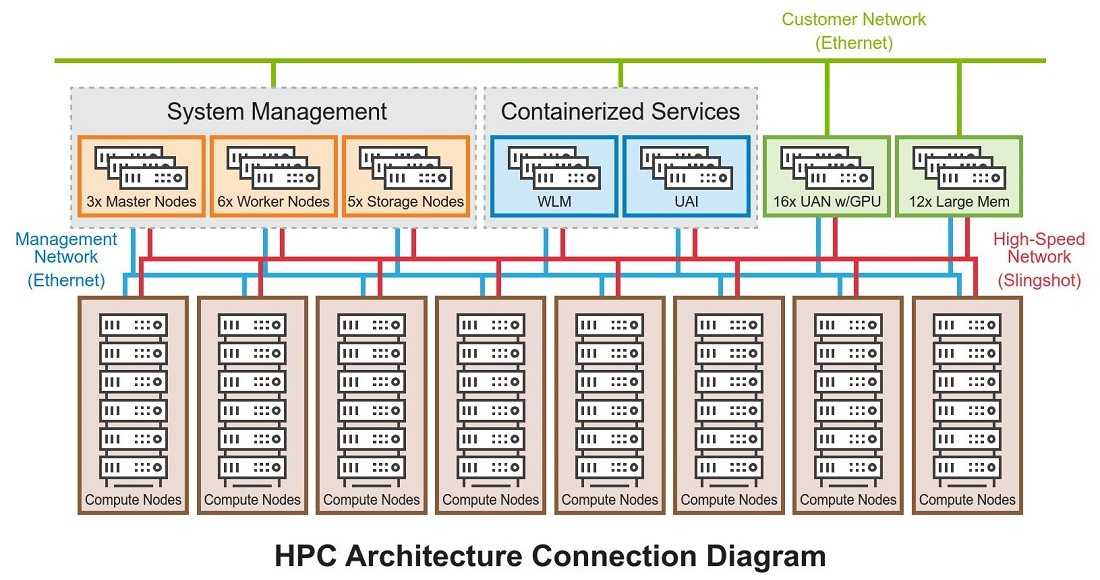
\includegraphics[scale=0.42]{images/hpc_cluster}
		\caption{Tomado de \url{https://www.gigabyte.com/Article/high-performance-computing-cluster}}
	\end{figure}
\end{frame}

\begin{frame}{¿Cómo se administra un Cluster con miles de nodos?}

\begin{columns}
\begin{column}{0.5\textwidth}
  \textbf{Herramientas de configuración automatizada}
  
  \begin{figure}
  	
\includegraphics[scale=0.3]{images/cfengine}
  	
\includegraphics[scale=0.3]{images/ansible}
  \end{figure}
\end{column}
\begin{column}{0.5\textwidth}  %%<--- here
  \textbf{Job Scheduler o Resource Management System(RMS)}
    \begin{figure}
  	
\includegraphics[scale=0.3]{images/slurm}
  	
\includegraphics[scale=0.3]{images/condor}
  \end{figure}
\end{column}
\end{columns}

\end{frame}



\begin{frame}{Dos visiones}
\begin{columns}
\begin{column}{0.5\textwidth}
  \textbf{Administradoras}
  
  Se aseguran que la clienta-usuaria tenga las herramientas y soporte necesario para el uso eficiente de los recursos.
  \begin{figure}
  	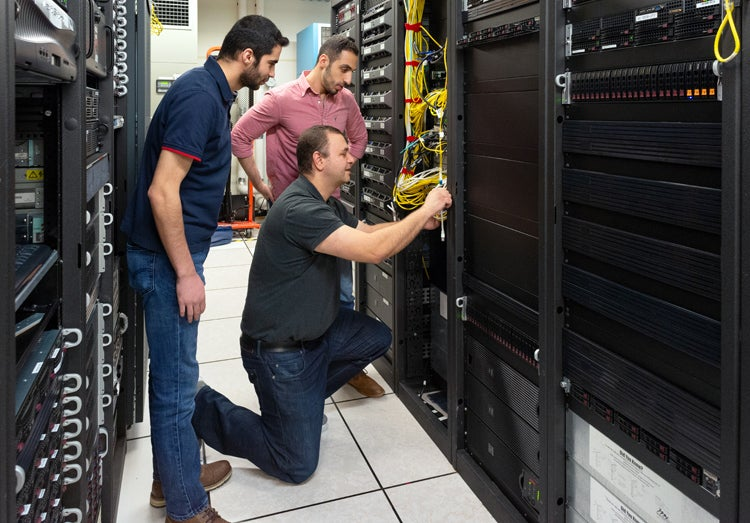
\includegraphics[scale=0.2]{images/sysadmin_humano}
  \end{figure}
\end{column}
\begin{column}{0.5\textwidth}  %%<--- here
  \textbf{Usuarias}
  
  Consume los recursos.
  \vspace{1.4cm}
    \begin{figure}
  	
\includegraphics[scale=0.65]{images/usuario_hpc}

  \end{figure}
\end{column}
\end{columns}
\end{frame}

\begin{frame}{Todo parece estar bien ... }
	\begin{figure}
		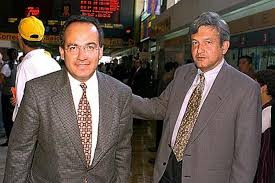
\includegraphics[scale=0.8]{images/armonia_cuatro	}
	\end{figure}
\end{frame}

\begin{frame}{La realidad es otra}
	\begin{figure}
		
\includegraphics[scale=0.3]{images/realidad}
	\end{figure}
\end{frame}


\begin{frame}{Problema}

	\begin{itemize}
		\item Como en todo aquello donde existe el uso de un recurso compartido, las relaciones Sysadmin-Usuaria, Usuaria-Usuaria no son siempre coordiales. 
		\item Hay conflicto : ¿Quién y cuándo tiene acceso al recurso?¿Hay asignación justa de recursos?¿Hay usuarios con mayores privilegios?
		\item \textbf{Sysadmin} : Definen \textbf{Reglas-Políticas de uso} con el objetivo de satisfacer las necesidades de las usuarias pero también acorde a las necesidades de mantener un recurso usable y confiable.
		\item \textbf{Usuaria} : Estas reglas y políticas se traduce en sistemas y software limitantes e inmóviles \citep{kurtzer2017singularity}. 
	\end{itemize}

\end{frame}

\begin{frame}{Problema}

	\begin{center}
		\textit{This static nature coupled with distribution-specific software builds meant that service providers would ultimately end up limiting the scope of computational science that their systems could support}\citep{kurtzer2017singularity}
	\end{center}

\end{frame}

\begin{frame}{Propuesta de solución\citep{kurtzer2017singularity}}
	\textbf{Ambientes portables}
	
	\begin{itemize}
		\item Máquinas virtuales.
		\item Contenedores.
	\end{itemize}
\end{frame}

\begin{frame}{Máquinas virtuales}

\begin{columns}
\begin{column}{0.5\textwidth}

  \begin{figure}
  	
\includegraphics[scale=0.3]{images/vmachines}
  \end{figure}
\end{column}
\begin{column}{0.5\textwidth}  %%<--- here

	Proporcionan un ambiente completo, incluyendo dependencias de software, bibliotecas, datos que pueden ser encapsulados y ejecutados donde sea.
	
	\begin{center}
		\textbf{Problema}
	\end{center}
	
Introduce una sobrecarga computacional considerable debido al nivel requerido de virtualización para emular el sistema operativo y el kernel.
\end{column}
\end{columns}
\end{frame}



\begin{frame}{Contenedores}
	\begin{columns}
\begin{column}{0.5\textwidth}

  \begin{figure}
  	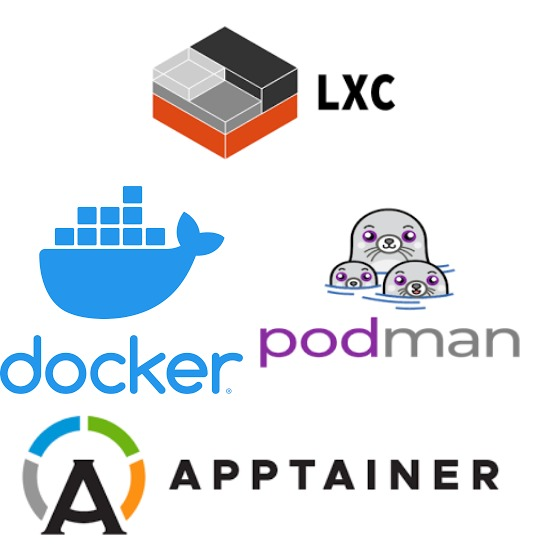
\includegraphics[scale=0.3]{images/contenedores_tecnologias}
  \end{figure}
\end{column}

	\vspace{-0.5cm}

\begin{column}{0.5\textwidth}  %%<--- here
	
	Características de virtualización ligera en el kernel de Linux hace posible construir virtualización más ligera. 

	\vspace{0.2cm}
	
	Las características específicas del kernel son las que se ocupan de aislar procesos, en particular \citep{nemeth2018unix}:
	
		\begin{itemize}
			\item \textbf{Namespaces} : aislan los procesos del contenedor desde la perspectiva de las características del sistema operativo.
			\item \textbf{Control groups (cgroups)} limita el uso de los recursos del sistema y prioriza ciertos procesos sobre otros.
					\end{itemize}

	
\end{column}
\end{columns}
\end{frame}


\begin{frame}{Apptainer}
  \begin{figure}
  	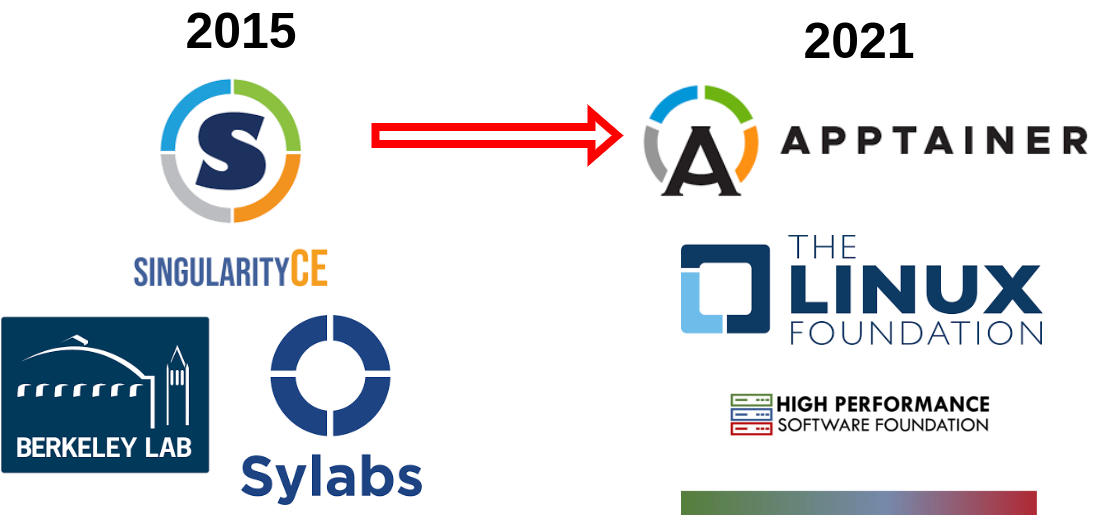
\includegraphics[scale=0.31]{images/apptainer_historia}
  \end{figure}
\end{frame}


\begin{frame}{Gregory Kurtzer}
  \begin{figure}
  	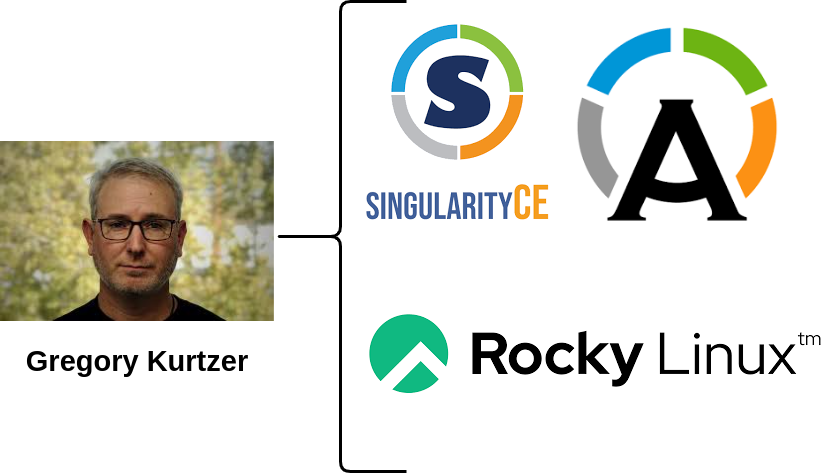
\includegraphics[scale=0.4]{images/kurtzer}
  \end{figure}
\end{frame}

\begin{frame}{Objetivos de Apptainer \citep{kurtzer2017singularity}}
  \begin{itemize}
  	\item \textbf{Mobility of compute} (\textbf{Portabilidad})
  	\item \textbf{Reproducibilidad}
  	\item \textbf{Soporte e integración con recursos tradicionales de HPC}
  \end{itemize}
\end{frame}


\begin{frame}{Mobility of compute}
  \begin{itemize}
  	\item Capacidad de definir, crear y mantener un workflow local que puede ser usado con confianza en diferentes hosts, sistemas operativos de Linux, provedores de servicios en la nube, etc.
  	\item Esencial para la \textit{ciencia reproducible}.
  	\item Apptainer usa un formato de imagen distribuible que encapsula el contenido completo del contenedor en un \textbf{archivo de imagen único} (archivo \textbf{.sif}).

  \end{itemize}
\end{frame}

\begin{frame}{Mobility of compute}
  \begin{itemize}
 	\item El archivo .sif es la representación completa de todos los archivos dentro del contenedo.
 	\item El .sif encapsula el sistema operativo así como también todas las dependencias necesarias para ejecutar un workflow definido.
  	\item Este archivo puede ser copiado, compartido, mejorado, además de seguir el estándar de permisos de UNIX.
  \end{itemize}
\end{frame}


\begin{frame}{Reproducibilidad}
  \begin{itemize}
  	\item Si se garantiza portabilidad, se garantiza reproducibilidad.
 
  	\item Una vez que se ha definido el workflow dentro de contenedor, el archivo .sif puede usarse con confianza que el código dentro del contenedor no ha sido modificado.
  	\item Apptainer utiliza un método de validación de integridad mediante un hash por SHA256 que garantiza que la imagen del contenedor que es distribuida no ha sido modificada. 
  	\item Cuando las investigadoras publican sus resultados, pueden distribuir el .sif de la imagen utilizada en el artículo así como su hash, permitiendo que alguien más pueda validar los resultados y confirmar la integridad del .sif descargado con el hash. 
  \end{itemize}
\end{frame}

\begin{frame}{Soporte e integración con recursos tradicionales de HPC}

Apptainer soporta de forma nativa tecnologías como :
	\begin{itemize}
		\item Infiniband y Lustre (comunicación en red de alta velocidad y baja latencia y sistema de archivos paralelo, respectivamente).
		\item SLURM, Torque, etc (Sistemas de administración de recursos).
		\item Aceleradores: GPUs, TPUs.
		\item Software tradicional de HPC: OpenMP, MPI. 
	\end{itemize}

Esto como resultado que Apptainer se ejecuta como cualquier otro comando del sistema. 
\end{frame}


\begin{frame}{Casos de Uso}

\textbf{Investigaciones académicas}

\begin{itemize}
	\item Desarrollan en ambiente local, escalan la ejecución en otra infraestructura.
	\item Publican resultados y distruyen el análisis completo y el workflow dentro de un .sif acompañado del hash, permitiendo la reproducción y validación de resultados. 
\end{itemize}
\end{frame}

\begin{frame}{Casos de Uso}

\textbf{Administración de sistemas}

\begin{itemize}
	\item El sistema de HPC es controlado y administrado por una administradora de sistemas y su equipo. 
	\item Para mantener el sistema seguro, sólo a este grupo se le concede acceso root y control sobre el estado del sistema operativo.
	\item Los usuarios del sistema no tiene acceso como root.
	\item Si un usuario puede escalar a root (incluso dentro de un contenedor) en el sistema, el usuario puede potencialmente hacer cosas malas (deliberadamente o no). 
\end{itemize}
\end{frame}

\begin{frame}{Casos de Uso}

\textbf{Administración de sistemas}

\begin{itemize}
	\item Para mitigar estos riesgos, Apptainer no proporciona la capacidad de escalar permisos dentro de contenedor.
	\item Con Apptainer \textbf{si un usuario no tiene acceso a root en el sistema objetivo, tampoco puede escalar privilegios como root dentro del contenedor}. 
	\item La sysadmin instruiría  a las usuarias a desarrollar sus imágenes en un sistema donde tengan acceso a root para realizar operaciones de escritura en las imágenes, para posteriormente transferirlas al cluster para su ejecución a gran escala.
\end{itemize}
\end{frame}

\begin{frame}{Casos de Uso}

\textbf{Eliminar redundancia en tecnologías de contenedores}

\begin{itemize}
	\item Es posible ejecutar imágenes de Docker en ambientes HPC con Apptainer.
	\item Por diseño, Apptainer ha sido desarrollado para trabajar sin problemas con Docker. 
\end{itemize}
\end{frame}

\begin{frame}{¿Por qué no sólo usar Docker en ambientes HPC?}

\begin{center}
	\textbf{Problemas de seguridad}
\end{center}

\begin{itemize}
	\item Para cada contenedor que Docker ejecuta, el proceso del contenedor es extendido como hijo del demonio de Docker que es propiedad de root. 
	\item Como la usuaria es capaz de interactuar y controlar el demonio de Docker, teóricamente es posible obligar al proceso del demonio a otorgar permisos privilegiados a la usuaria\footnote{ Uno de los principales retos en los centros HPC dedicados a la investigación es permitir a las usuarias ejecutar código arbitrario manteniendo simultaneamente que el sistema no se encuentra comprometido por código malicioso (intencionalmente malicioso o no).}.
\end{itemize}

\end{frame}

\begin{frame}{Workflow de Apptainer}
	\begin{itemize}
		\item \textbf{Build}. Construye el contenedor de Apptainer en un sistema local donde tengas acceso a root o sudo.
		\item \textbf{Transfer}. Transfiere el contenedor a un sistema HPC donde quieres ejecutarlo.
		\item \textbf{Run}. Ejecuta el contenedor en el sistema HPC.
	\end{itemize}
\end{frame}

\begin{frame}[allowframebreaks]
        \frametitle{References}
		\bibliographystyle{apalike}

       \bibliography{apptainer_virtualizacion.bib}
\end{frame}



\end{document}